\subsection{Allee效应可以给疾病传播的一些概念一些启示}
\begin{frame}{Allee效应可以给疾病传播的一些概念一些启示}
    \begin{itemize}
        \item 传统的流行病学模型,如SIS、SIR和SEIR模型中,交互强度的假设都依赖于人口密度。关停人流密集场所的效果相当于降低最大密度区域的人口密度。
        \item 这同时会带来新的高密度地区,如\textbf{小区}、等。
        \pause
        \item critical community size (CCS)
        \begin{itemize}
            \item Bartlett, M. (1960). The Critical Community Size for Measles in the United States. Journal of the Royal Statistical Society. Series A (General), 123(1), 37-44. doi:10.2307/2343186 \href{https://www.jstor.org/stable/pdf/2343186.pdf?refreqid=excelsior\%3A8b718b75a5e4633091a524237af85adf}{PDF链接}
        \end{itemize}
        \item 随着城市化的推进和高层建筑的增加,该概念可能是时候该重新定义了。
    \end{itemize}
\end{frame}

\subsection{城市空间异质性的一种新解释:临界交互密度}

\begin{frame}{城市空间异质性的一种新解释:临界交互密度}
    本次抗疫过程中,群体层面主要的限制手段是限制个体出行。实际作用是减小了大部分人的活动半径。需要注意的是,该措施同时会使得局部交互有较大提升。本研究试图探究缩小活动尺度带来的非线性效应。
    
    \vspace{0.5cm}
    
    我们提出了一个基于复杂人口分布的SIER模型,该模型中,每个结点的人口数将不再固定,每个结点的状态将由总人口和患病人口比例两个量来决定。传播规律除了结点间传播之外,还有结点内的高速传播,以模拟小区传播的过程。
    
    \vspace{0.5cm}
    
    在人口的高度异质性假设下,本研究试图证明限制出行并不一定是最优解,而是在小区传播出现之前/患病比例比较低的时期的较优解。%在某些时期,流行病传播与出行限制关系不大。
\end{frame}

\begin{frame}{城市空间异质性的一种新解释:临界交互密度}
    与Allee效应的联系
    \begin{figure}
        \centering
        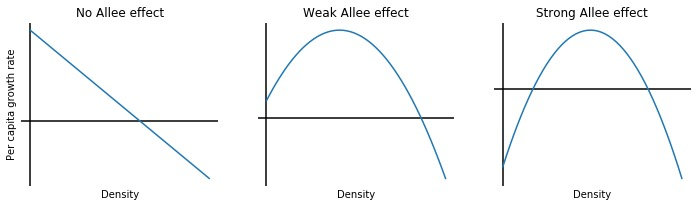
\includegraphics[width = 0.8\linewidth]{pics/allee.jpg}
    \end{figure}
\end{frame}

\begin{frame}{Model}
    我们首先抽象一下疾病在城市空间内交互的模式:
    \begin{itemize}
        \item 城市空间用$L\times L$的方格表示,每个格子上的residential人口是一个常数$a_{ij} = s_{ij}+i_{ij}+r_{ij}$, 格子之间的交互用矩阵$M_{L^2\times L^2}$来表示(要求$M_{kk} > \delta \sum_l M_{kl}$, $\delta$是一个大于$0$的常数);
        \item 假设交互对每对人是同质的:任意两个人一次接触产生传染的概率都相等,为$\mu$; 
        \begin{itemize}
            \item \textcolor{red}{作为两个地块$a,b$,产生疾病传播的期望数为$\mu (s_a i_b + s_b i_a)$}
        \end{itemize}
        \item 每个患病个体恢复的时间都是$r$; 
        \item (为了易于收敛,我们不妨假设恢复之后的个体都具有免疫力).
    \end{itemize}
\end{frame}

\begin{frame}{Insight}
    \begin{itemize}
        \item 由于有患病的因素存在,城市地块之间的交互是\textbf{非对称的},有\textbf{交配}的性质;
        \item 人口密集处处于高危险状态的概率较高,如果有疫情,在人口密集处优先出现疫情的概率比较大。
        \item 局部链接本身很强($M_{kk} > \delta \sum_l M_{kl}$), 限制出行后会更强,同时会出现新的人口密集处。
    \end{itemize}
    量化模型:\[\lambda_{n+1} = \beta_n S_n (I_n + \theta_n)^\alpha\]
    \begin{itemize}
        \item 其中,$n$为时刻,$\beta_n$是局部传染率,$\alpha$是混合率,$\theta_n$是(随机)接触率,假设是泊松分布$\text{Poi}(m\bar{I}_n).$的,$m$是空间耦合率,$\bar{I_n}$是上一个时刻邻居们染病的数量。这样的话,疾病生灭过程就由下面的负二项分布刻画:\[I_{n+1} \sim NegBin(\lambda_{n+1},I_n).\]
    \end{itemize}
\end{frame}

\begin{frame}{Insight}
    \begin{itemize}
        \item 这样非对称会出现时间上的不同步性,由于现代城市的发展,CCS (Critical Community Size) 可能会在城市内部出现。镶嵌结构可能会在城市内部出现。
        \item 高密度地块可能会长期留存病毒,并且容易产生新的爆发。
        \item 防疫时,除了切分地块,注意降低地块上人口密度亦是问题关键。
    \end{itemize}
    
\end{frame}

\begin{frame}{通勤模式对城市空间中疾病传播的影响}
    \begin{figure}
        \centering
        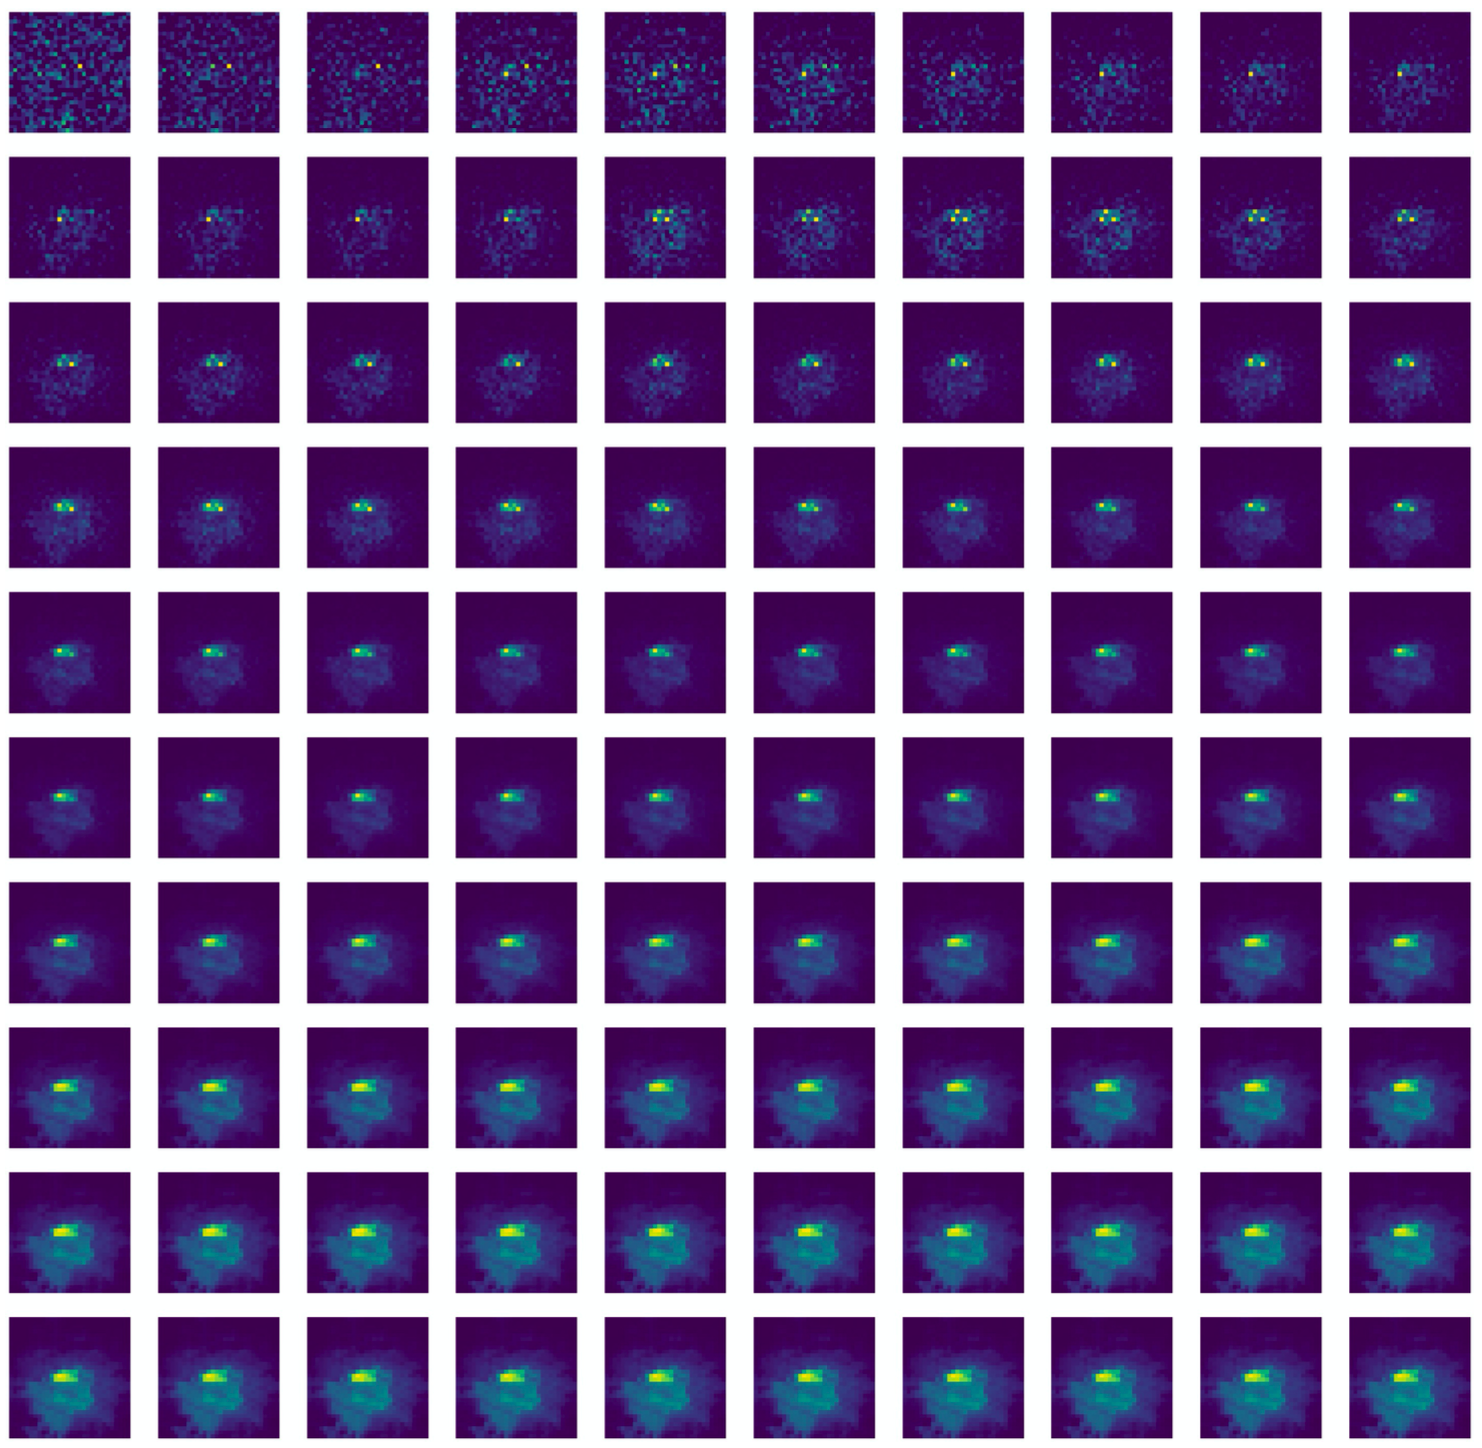
\includegraphics[width = 0.5\linewidth]{pics/simu.png}
        \caption{A simulation}
    \end{figure}
\end{frame}